% Capítulo 3
\chapter{Arquitetura}

ARASH (Robô Antropomórfico Aumentado com Sentido de Ser Humano), é um robô humanoide de 7,5 Kg, 1 metro de altura. Com 20 graus de liberdade (ou DOF, de \textit{degrees of freedom}), distribuídos em 6 DOF para cada perna, 3 em cada braço e 2 no pescoço.

Na arquitetura do sistema original (antes das mudanças propostas), existem 3 camadas principais que podem ser descritas independentemente: A camada de software, a camada de software de baixo nível, e a camada de hardware.

\todo{Nem todas as conexões numeradas são relevantes. Removo-as?}\begin{figure}[htb]
	\centering
	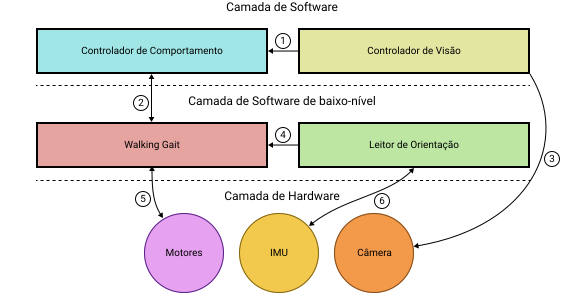
\includegraphics[scale=1]{imagens/svg/software-architecture}
	\textsf{\caption{Visão simplificada da arquitetura do sistema.}}
	\label{fig:SoftwareArchitecture-SimplifiedOverview}
\end{figure}

A camada de software é executada dentro do ``controlador principal'', que é um computador \textit{mini-box PC MAXData QutePC-3001} com um processador 64 bits de dois núcleos Intel\copyright{} Celeron\copyright{} 847E (1,1GHz e 2MB de \textit{cache}), rodando o Ubuntu 14.04. Esta camada é responsável por rodar os componentes de software e enviar comandos de controle para a camada inferior de baixo nível, conexão \circled{2}. Por exemplo, durante uma partida de futebol, o programa ``jogador'' ativa o sistema de visão, que localiza a bola em relação ao robô e retorna a informação ao ``jogador'', que envia o comando de controle ao \textit{walking gait} para caminhar a metade da velocidade total à frente com 32\degree{} à esquerda.

A camada de software de baixo nível é responsável pelo processamento de dados da IMU, juntamente com a execução do \textit{walking gait}. Esta camada roda dentro da placa microcontroladora \textit{Robotis.Co OpenCM9.04} (com um processador \textit{32bit ARM Cortex-M3}, memória \textit{flash} de 128Kb e 20Kb de \textit{SRAM}), \textit{arduino-like}. Esta camada roda o \textit{walking gait} e o \textit{sistema de orientação}. Ela tem acesso direto a enviar e receber comandos dos motores (conexão \circled{5}) e os sensores da \textit{IMU} (conexão \circled{6}), conectando-se ao controlador principal via USB (conexão \circled{2}) recebendo pacotes de controle e enviando comandos para os motores em uma conexão \textit{TTL} \textit{half-duplex} a 1 Mbps.

O \textit{walking gait} monitora a USB aguardando os comandos de controle que contém as velocidades da caminhada, enviados a partir do controlador principal. Já o componente leitor de orientação desempenha um papel importante dentro do \textit{walking gait}. Ele é o responsável pela verificação da orientação da rotação do torso, uma vez que a IMU está situada nas costas de Arash, em relação ao eixo da gravidade. Desta forma, o \textit{walking gait} faz correções nas juntas para compensar um eventual desvio na trajetória. Mais detalhes sobre a implementação deste componente serão descritos \todo{Referênciar seção especifica}nos próximos capítulos!!!

Na design original do time AUT-UofM, a \textit{OpenCM9.04} é responsável por executar o componente de caminhada, coordenando os movimentos das juntas de acordo com parâmetros recebidos através da USB (enviados pelo controlador principal). Desta forma, os dados de leitura sobre a posição das juntas ou sobre a orientação, obtido pelos sensores da IMU, não são necessários fora da placa microcontroladora.

\subsection{Graus de Liberdade e Atuadores}

Em Arash, todos os atuadores são produzidos pela Robotics.Co. Porém, devido a variação de carga nas diversas juntas, foram utilizados modelos diferentes da mesma série MX, esta opção diminui o custo final do robô.

Tão importante quanto a configuração das juntas é a orientação dos atuadores para que os cálculos funcionem como o esperado.

\begin{figure}[htb]
	\centering
	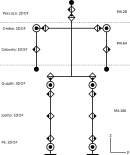
\includegraphics[scale=0.6]{imagens/svg/arash-schematics}
	\textsf{\caption{Esquema de orientação dos atuadores de Arash}}
	\label{fig:ArashSchematics}
\end{figure}

Na figura acima, podemos observar o esquema de orientação dos atuadores em cada junta. No diagrama encontram-se 4 símbolos com significados diferentes:

O pequeno círculo preto preenchido, representa apenas o fim de cadeia. Assim, estes símbolos representam as mãos, que não possuem atuadores, e a ponta da cabeça, onde fica apenas a câmera. Adicionalmente, os "círculo vazado com outro círculo preto preenchido dentro" e os diamantes representam atuadores.

No caso do "círculo vazado com outro círculo preto preenchido dentro", o atuador será referenciado como "frontal" e propicia rotação orientada pelo eixo X (no plano YZ), que está aponta para o leitor (para fora do papel).

Nos diamantes, o atuador está apontando para a marcação preta na ponta do diamante. Atuadores que apontam para direita ou esquerda, são chamados de horizontais. Eles apresentação rotação com base no eixo Y. Já os que apontam para cima ou baixo são chamados de atuadores transversais que representação transformações na rotação no eixo Z.

\todo{Ordem imagens confusa!?}
\begin{figure}[htb]
	\centering
	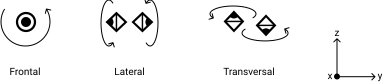
\includegraphics[scale=0.6]{imagens/svg/actuators-orientation}
	\textsf{\caption{Sentido do movimentos dos atuadores}}
	\label{fig:ActuatorsOrientation}
\end{figure}

\todo{Referenciar ao paper de descrição de Arash}
Estas orientações são importantes durante os cálculos dos ângulos enviados às juntas. Por exemplo, caso a orientação do cotovelo esteja trocada, no cálculo ou no robô real, qualquer ângulo enviado a ele resultará em uma rotação para trás, um movimento que o cotovelo humano não é capaz de realizar.

\todo{Conectar estes dois parágrafos}
No pescoço, onde a carga é bem leve, 'MX-28' são suficientes. Dois atuadores, um na posição transversal (o atuador mais baixo) que fornece o movimento panorâmico a cabeça e outro na posição horizontal, fornecendo o movimento de inclinação vertical da cabeça.

Nos braços, que podem sofrer uma carga maior, atuadores 'MX-64' são utilizados. Isso é importante já que existem modalidades de competições, como o levantamento de peso, que testam a capacidade do carregamento de cargas.

Para as pernas, foram utilizados atuadores 'MX-106' que são mais poderosos que os anteriores. Entretanto, na fase de projeto, simulações mostraram que durante o movimento de levantar-se do chão (em caso da recuperação de uma possível queda), o torque nas juntas do joelho era levado ao máximo suportado pelo 'MX-106', podendo assim levar este motor à falha. Desta forma, 2 atuadores sincronizados passaram a formar esta junta, afim de proporcionar um maior torque para os movimentos necessários. Esta junta dupla não oferece nenhum impacto na implementação, já que os motores da série 'MX-106' oferecem a capacidade de serem ligados e sincronizados via \textit{hardware} - assim, a nível de software, controla-se apenas 1 único atuador. Desta forma, apesar das 20 DOF, Arash possui 22 motores.

\section{Arquitetura de Software pré-solução}



\section{Modificações na \textit{OpenCM9.04}}

Na implementação da solução deste trabalho a geração das trajetórias do \textit{walking gait} será transferida da \textit{OpenCM9.04} para o controlador principal. Entretanto, a placa microcontroladora ainda terá um papel crucial dentro da nova implementação.


\begin{guide}
Detalhar arquitetura.
\end{guide}

\begin{guide}
Detalhar componentes.
\end{guide}


\begin{itemize}
   \item ser claro, preciso, direto, objetivo e conciso, utilizando frases
   curtas e evitando ordens inversas desnecessárias;
   \item construir períodos com no máximo duas ou três linhas, bem como
   parágrafos com cinco linhas cheias, em média, e no máximo oito (ou seja, não
   construir parágrafos e períodos muito longos, pois isso cansa o(s) leitor(es)
   e pode fazer com que ele(s) percam a linha de raciocínio desenvolvida);
   \item a simplicidade deve ser condição essencial do texto; a simplicidade do
   texto não implica necessariamente repetição de formas e frases desgastadas,
   uso exagerado de voz passiva (como \textit{será iniciado}, \textit{será
   realizado}), pobreza vocabular etc. Com palavras conhecidas de todos, é
   possível escrever de maneira original e criativa e produzir frases elegantes,
   variadas, fluentes e bem alinhavadas;
   \item adotar como norma a ordem direta, por ser aquela que conduz mais
   facilmente o leitor à essência do texto, dispensando detalhes irrelevantes e
   indo diretamente ao que interessa, sem ``rodeios'' (verborragias);
   \item não começar períodos ou parágrafos seguidos com a mesma palavra, nem
   usar repetidamente a mesma estrutura de frase;
   \item desprezar as longas descrições e relatar o fato no menor número
   possível de palavras;
   \item recorrer aos termos técnicos somente quando absolutamente
   indispensáveis e nesse caso colocar o seu significado entre parênteses (ou
   seja, não se deve admitir que todos os que lerão o trabalho já dispõem de
   algum conhecimento desenvolvido no mesmo);
   \item dispensar palavras e formas empoladas ou rebuscadas, que tentem
   transmitir ao leitor mera ideia de erudição (até mesmo às vezes ilusória);
   \item não perder de vista o universo vocabular do leitor, adotando a seguinte
   regra prática: \textit{nunca escrever o que não se diria};
   \item termos coloquiais ou de gíria devem ser usados com extrema necessidade
   (ou mesmo nem serem utilizados) e apenas em casos muito especiais, para não
   darem ao leitor a ideia de vulgaridade e descaracterizar o trabalho;
   \item ser rigoroso na escolha das palavras do texto, desconfiando dos
   sinônimos perfeitos ou de termos que sirvam para todas as ocasiões; em geral,
   há uma palavra para definir uma situação;
   \item encadear o assunto de maneira suave e harmoniosa, evitando a criação de
   um texto onde os parágrafos se sucedem uns aos outros como compartimentos
   estanques, sem nenhuma fluência entre si;
   \item ter um extremo cuidado durante a redação do texto, principalmente com
   relação às regras gramaticais e ortográficas da língua; geralmente todo o
   texto é escrito na forma impessoal do verbo, não se utilizando, portanto, de
   termos em primeira pessoa, seja do plural ou do singular.
\end{itemize}

Continução do texto.


\section{Seção 1}

Teste de tabela.

\begin{table}[!htb]
   \textsf{\caption{Tabela sem sentido.}}
   \centering
   \medskip
   \begin{tabular}{c|p{4cm}}
      \hline
      \textbf{Título Coluna 1} & \textbf{Título Coluna 2} \\
      \hline
      Texto curto & Texto mais extenso, que requer mais de uma linha \\
      \hline
      \label{tab:TabelaSemSentido}
   \end{tabular}
\end{table}


\section{Seção 2}

Seção 2


\subsection{Subseção 2.1}

Referência à tabela definida no início: \ref{tab:TabelaSemSentido}


\subsection{Subseção 2.2}

Texto a ser enumerado.

\begin{enumerate}
   \item Item 1
   \item Item 2, com nota explicativa\footnote{Nota explicativa}
   \item Item 3
\end{enumerate}


\section{Seção 3}

Texto antes de equação.

\begin{equation}
   x = y + z
\end{equation}

Outra maneira de se usar equação.

$ \forall \pi : \pi \hookrightarrow \gamma $

Texto depois de equação.

\section{Seção 4}

Exemplo de código
